%%%%%%%%%%%%%%%%%%%%%%%%%%%%%%%%%%%%%%%%%%%%%%%%
%% Compile the master file!
%% 		Slides: Stefan Müller
%% 		Course: GK Linguistik
%%%%%%%%%%%%%%%%%%%%%%%%%%%%%%%%%%%%%%%%%%%%%%%%

%% -*- coding:utf-8 -*-

\iftoggle{ba-linguistik}{
\title{Grundkurs Linguistik}

\subtitle{Syntax}

\author{
	{Stefan Müller}
%	\\
%	{\footnotesize \url{http://www.linguistik.hu-berlin.de/staff/amyp}\\
%	\href{mailto:mapriema@hu-berlin.de}{mapriema@hu-berlin.de}}
}

\institute{Institut für deutsche Sprache und Linguistik}

%%%%%%%%%%%%%%%%%%%%%%%%%      
\date{ }
%\publishers{\textbf{6. linguistischer Methodenworkshop \\ Humboldt-Universität zu Berlin}}

%\hyphenation{nobreak}


%%%%%%%%%%%%%%%%%%%%%%%%%%%%%%%%%%%%%%%%%%%%%%%%%%%%
%%%             Preamble's End                   %%%
%%%%%%%%%%%%%%%%%%%%%%%%%%%%%%%%%%%%%%%%%%%%%%%%%%%%      


\huberlintitlepage[22pt]
}

\section{Syntax}
\author{Stefan Müller}


\iftoggle{ba-linguistik}{




\frame{
\frametitle{Lach Dich schlapp!}

\vfill

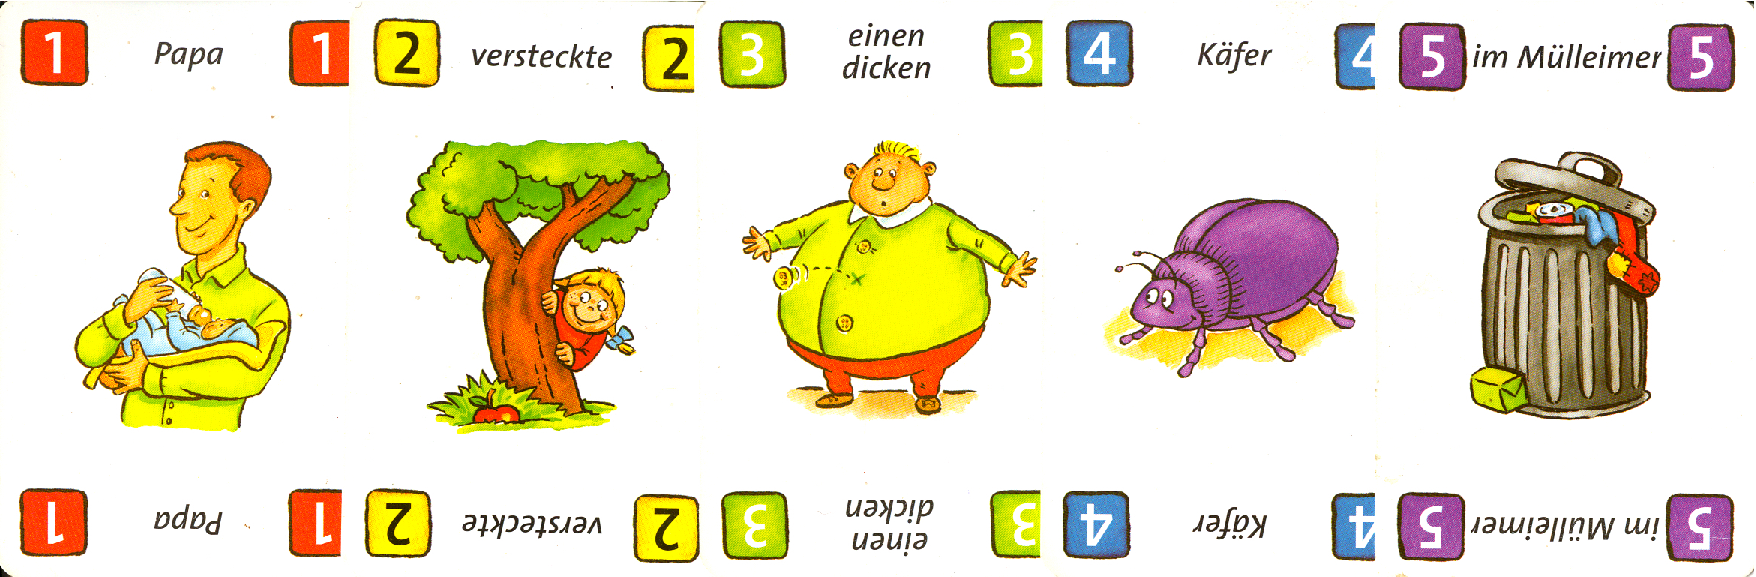
\includegraphics[width=\textwidth]{Bilder/lach-dich-schlapp-pappa-versteckte}

\vfill
Reihe die Spielkarten in der Reihenfolge 1 bis 5 aneinander.

\vfill
\footnotesize{(Ravensburger, 6--12 Jahre)}

}
\frame{
\frametitle{Lach Dich schlapp!}

\vfill
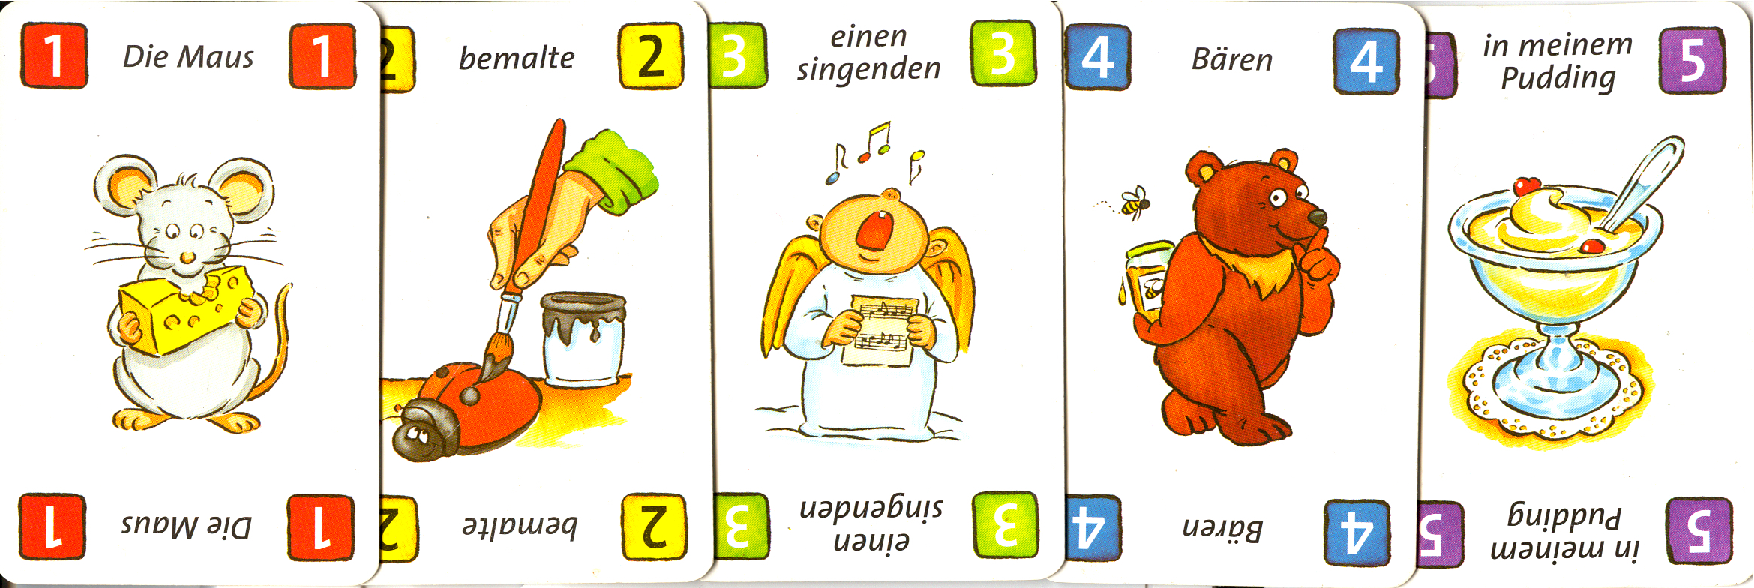
\includegraphics[width=\textwidth]{Bilder/lach-dich-schlapp-die-maus-bemalte}

\vfill
Warum funktioniert das Spiel?

\vfill
}


\frame{
\frametitle{Form und Bedeutung}


\begin{tabular}{@{}llll@{}}
{}[Papa]     & [versteckte] & [einen dicken Käfer]    & [im Mülleimer].\\
{}[Die Maus] & [bemalte]    & [einen singenden Bären] & [in meinem Pudding].
\end{tabular}

\bigskip

\begin{itemize}
\item Wir können die Blöcke austauschen und die Sätze bleiben wohlgeformt.

\item Allerdings passt die Bedeutung im zweiten Beispiel nicht mehr.

\pause

\item Zusammensetzung von Einheiten und Umordnung = \blaubf{Syntax}

\pause

\item Bedeutung im engeren und weiteren Sinn = \blaubf{Semantik}/\blaubf{Pragmatik}

\end{itemize}

}

%% \frame{
%% \frametitle{Verschwende Deine Jugend!}

%% \vfill
%% \centerline{\includegraphics[width=0.8\textwidth]{Bilder/daf}}

%% \vfill
%% }


%% \frame{
%% \frametitle{Spiel und Spaß}


%% Als kleiner Junge war mir schon klar: mein Leben wird ganz wunderbar.\\
%% Ich lebe einfach  radikal, nach Algorithmen meiner Wahl.\\
%% Ich richt' mein Leben radikal, nach Algorithmen meiner Wahl.\\
%% Ein Algorithmus ist ein Ball, darin gefangen eine Zahl.\\
%% Befrei die Zahl und spiel den Ball. Spiel den Ball.

%% D.A.F.: Fünfzehn neue DAF-Lieder, Superstar Recordings, 2003

%% \bigskip

%% Syntax = Spiel\\
%% Semantik = Spaß



%% }

}


\frame{
\frametitle{Syntax: Material}

\begin{itemize}
\item Müller, 2013. Grammatiktheorie. Tübingen: Stauffenburg-Verlag, Kapitel~1--2.\nocite{MuellerGTBuch2}


\url{https://hpsg.hu-berlin.de/~stefan/Pub/grammatiktheorie.html}

\pause
\item Oder auf Englisch: \url{http://langsci-press.org/catalog/book/195}


\bigskip

Zur Vorbereitung bitte immer entsprechende Abschnitte lesen! 

%\pause

%\item Im Sprachbeschreibungsteil werden wir \citew{Duden2009a} verwenden.
\end{itemize}

}

\exewidth{(370)}






\iftoggle{syntaxvorlesungen}{

\frame{
\frametitle{Alte Weisheit}

{}[Grammatik ist] das Tor zur Freiheit, die Medizin für die Krankheiten der Sprache, der Reiniger
aller Wissenschaften; sie verbreitet ihr Licht über ihnen; \ldots sie ist
die erste Sprosse auf der Leiter, die zur Realisierung übernatürlicher Kräfte führt und der
gerade, königliche Weg für diejenigen, die die Freiheit suchen. (Bhartrhari, Spruchdichter,
gest.\ vor 650 n. Chr., aus \emph{Vakyapadiya}, gefunden von Gabriele Knoll)

}
}

%\if 0

\iftoggle{einfsprachwiss-exclude}{
\section{Einleitung}
}

\iftoggle{hpsgvorlesung}{
\outline{

\begin{itemize}
\item Wozu Syntax? / Phrasenstrukturgrammatiken
\item Formalismus
\item Valenz und Grammatikregeln
\item Komplementation
\item Semantik
\item Adjunktion und Spezifikation
\item Das Lexikon: Typen und Lexikonregeln
\item Topologie des deutschen Satzes
\item Konstituentenreihenfolge
\item Nichtlokale Abhängigkeiten
\item Relativsätze
\item Lokalität
%\item Komplexe Prädikate: Der Verbalkomplex
\end{itemize}
}
}%\end{hpsgvorlesung}


\iftoggle{einfsprachwiss-exclude}{
\frame{
\frametitlefit{Motivation fromale Syntax und Phrasenstrukturgrammatiken}

\begin{itemize}
\item Literatur: \citew[Kapitel~1]{MuellerLehrbuch3} bzw.\ \citew[Kapitel~1]{MuellerGTBuch2}
\item Englische Version des Grammatiktheoriebuches: \citew{MuellerGT-Eng1}
\end{itemize}

\vspace{1cm}

%%\rotbf{Achtung, wichtiger Hinweis: Diese Literaturangabe hier bedeutet,\\dass Sie die Literatur zum
%%   nächsten Mal lesen sollen!!!!}
%% }
}
}%\end{einfsprachwiss-exclude}


\subsection{Wozu Syntax?}



\frame{
\frametitle{Wozu Syntax?}

\begin{itemize}
\item Literatur: \citew[Kapitel~1]{MuellerLehrbuch3} bzw.\ \citew[Kapitel~1]{MuellerGTBuch2}
\medskip

\item Zeichen: Form-Bedeutungs-Paare \citep{Saussure16a}
\pause
\item Wörter, Wortgruppen, Sätze
\pause
\item Sprache $\stackrel{?}{=}$ endliche Aufzählung von Wortfolgen\\
\pause
      Sprache ist endlich, wenn man maximale Satzlänge annimmt
      \eal
      \ex Dieser Satz geht weiter und weiter und weiter und weiter \ldots
\pause
      \ex {}[Ein Satz ist ein Satz] ist ein Satz.
      \zl
\pause
      extrem viele Sätze, Beschränkung der Wiederholung willkürlich

\item Unterscheidung zwischen \alert{Kompetenz} (das Wissen darüber, was geht) und
  \alert{Performanz} (der Benutzung des Wissens)

\end{itemize}
}


\frame{
\frametitle{Die Kinder von Bullerbü}

Und wir beeilten uns, den Jungen zu erzählen, wir hätten von Anfang an gewußt, daß es nur eine
Erfindung von Lasse gewesen sei. Und da sagte Lasse, die Jungen hätten gewußt, daß wir gewußt
hätten, es sei nur eine Erfindung von ihm. Das war natürlich gelogen, aber vorsichtshalber sagten
wir, wir hätten gewußt, die Jungen hätten gewußt, daß wir gewußt hätten, es sei nur eine Erfindung
von Lasse. Und da sagten die Jungen -- ja -- jetzt schaffe ich es nicht mehr aufzuzählen, aber es
waren so viele "`gewußt"', daß man ganz verwirrt davon werden konnte, wenn man es hörte. (S.\,248)

\bigskip

Wir sind prinzipiell in der Lage, komplexere Sätze zu bilden (Kompetenz), aber irgendwann werden wir
verwirrt, weil unsere Gehirne nicht mehr mitmachen (Performanz).


}




\frame{
\frametitle{Kreativität}


\begin{itemize}
\item Wir können Sätze bilden, die wir noch nie gehört haben $\to$\\
      muss Strukturierung, Muster geben

\end{itemize}


}

\frame{
\frametitle{Direkte Evidenz für syntaktische Strukturen?}

\begin{itemize}
\item Wir können feststellen, dass wir Regeln verwenden,\\
      indem wir Kinder beobachten.
      
      Kinder wenden Regeln mitunter falsch an (bzw. eben ihre eigenen Regeln).

\pause
\item Beispiel aus der Morphologie:
\eal
\ex[*]{
die Baggers
}
\ex[*]{
die Ritters
}
\zl
\end{itemize}
}


\frame{
\frametitle{Wozu Syntax? Bedeutung aus Bestandteilen ermitteln}

\begin{itemize}
\item Bedeutung einer Äußerung aus den Bedeutungen ihrer Teile bestimmen
      \ea
      Der Mann kennt diese Frau.
      \z
\pause
\item Syntax: Art und Weise der Kombination, Strukturierung 
      \eal
      \ex Die Frau kennt die Mädchen.
      \ex Die Frau kennen die Mädchen.
\pause
      \ex Die Frau schläft.
      \ex Die Mädchen schlafen.
      \zl
        Subjekt-Verb-Kongruenz $\to$ Bedeutung von (\mex{0}a,b) ist eindeutig
\end{itemize}

}

\subsection{Warum formal?}
\frame[shrink=20]{
\frametitle{Warum formal?}


Precisely constructed models for linguistic structure can play an
important role, both negative and positive, in the process of discovery 
itself. By pushing a precise but inadequate formulation to
an unacceptable conclusion, we can often expose the exact source
of this inadequacy and, consequently, gain a deeper understanding
of the linguistic data. More positively, a formalized theory may 
automatically provide solutions for many problems other than those
for which it was explicitly designed. Obscure and intuition-bound
notions can neither lead to absurd conclusions nor provide new and
correct ones, and hence they fail to be useful in two important respects. 
I think that some of those linguists who have questioned
the value of precise and technical development of linguistic theory
have failed to recognize the productive potential in the method
of rigorously stating a proposed theory and applying it strictly to
linguistic material with no attempt to avoid unacceptable conclusions by ad hoc adjustments or loose formulation.
\citep[S.\,5]{Chomsky57a}


As is frequently pointed out but cannot be overemphasized, an important goal
of formalization in linguistics is to enable subsequent researchers to see the defects
of an analysis as clearly as its merits; only then can progress be made efficiently.
\citep[S.\,322]{Dowty79a}


\bigskip

\begin{itemize}
\item Was bedeutet eine Analyse genau?
\item Welche Vorhersagen macht sie?
\item Ausschluß anderer Analysen
\end{itemize}


}

% has to be set elsewhere since this file is included into the syntax vorlesung
%\exewidth{(35)}

\subsection{Konstituenz}

\subsubsection{Konstituententests}

\frame{
\frametitle{Einteilung in Einheiten}

\begin{itemize}
\item Sätze können Sätze enthalten, die Sätze enthalten, die \ldots:
\ea
dass Max glaubt, [dass Julius weiß, [dass Otto behauptet, [dass Karl vermutet, [dass Richard bestätigt,
[dass Friederike lacht]]]]]
\z

Das funktioniert wie eine Matrjoschka bzw.\ wie eine Zwiebel.

\pause

\item Genauso kann man in (\mex{1}) Wörter zu Einheiten zusammenfassen:
\ea
Alle Studenten lesen während dieser Zeit Bücher.
\z

Welche?

\end{itemize}


}

\frame{
\frametitle{Schachteln}

\oneline{%
\begin{pspicture}(0,0)(12,1.8)
     \rput[bl](0,0){%
\psset{fillstyle=solid, framearc=0.25,framesep=5pt}
\psframebox{%
\psframebox{%
       \psframebox{alle}
       \psframebox{Studenten}}
\psframebox{lesen}
\psframebox{%
       \psframebox{während}
       \psframebox{%
           \psframebox{dieser}
           \psframebox{Zeit}}}
\psframebox{Bücher}}}
%\psgrid
    \end{pspicture}}

Wir tun alle Wörter, die zusammengehören, in eine Schachtel. 

Diese Schachteln können wieder in andere Schachteln getan werden.

Im Beispiel ist intuitiv klar, was zusammengehört, aber gibt es Tests?

}


\frame{
\frametitle{Konstituenz}

Begriffe:
\begin{description}
\item[Wortfolge]  Eine beliebige linear zusammenhängende Folge von Wörtern,\\
                  die nicht unbedingt syntaktisch oder semantisch zusammengehörig sein müssen.
\item[Wortgruppe, Konstituente, Phrase] Ein Wort oder mehrere Wörter,\\
                  die eine strukturelle Einheit bilden.
\end{description}


}

\iftoggle{syntaxvorlesungen}{
\frame{
\frametitle{Konstituententests}

Welche kennen Sie?
\pause

\begin{itemize}
\item Substituierbarkeit/Pronominalisierungstest/Fragetest
\item Weglaßtest
\item Verschiebetest (Umstelltest)
\item Koordinationstest
\end{itemize}


}
}%\end{syntaxvorlesungen}


\frame{
\frametitle{Konstituententests (I)}


\begin{description}
\item[Substituierbarkeit]
        Kann man eine Wortfolge einer bestimmten
	Kategorie in einem Satz gegen eine andere Wortfolge so austauschen, dass
	wieder ein akzeptabler Satz entsteht, so ist das ein Indiz dafür, dass 
	die beiden Wortfolgen Konstituenten bilden.
        \eal
        \ex Er kennt den Mann.
        \ex Er kennt eine Frau.
        \zl
\pause
\item[Pronominalisierungstest]
        Alles, worauf man sich mit einem Pronomen beziehen
	kann, ist eine Konstituente.
        \eal
        \ex Der Mann schläft.
        \ex Er schläft.
        \zl
%
\end{description}

}

\frame{
\frametitle{Konstituententests (II)}

\begin{description}
\item[Fragetest]
        Was sich erfragen läßt, ist eine Konstituente.
        \eal
        \ex Der Mann arbeitet.
        \ex Wer arbeitet?
        \zl
\pause
\item[Verschiebetest] Wortfolgen, die man ohne Beeinträchtigung der
	Korrektheit des Satzes verschieben bzw.\ umstellen kann, bilden eine Konstituente.
        \eal
        \ex weil keiner diese Frau kennt.
        \ex weil diese Frau keiner kennt.
        \zl
\pause
\item[Koordinationstest]
        Was sich koordinieren läßt, ist eine Konstituente.
        \ea
        Der Mann und die Frau arbeiten.
        \z
\end{description}

}



\iftoggle{konstituentenprobleme}{
\subsubsection{Bemerkungen zum Status der Tests}

\frame{
\frametitle{Bemerkungen zum Status der Tests: Expletiva (I)}

Was ist mit \emph{es} in (\mex{1})?
\ea
Es regnet.
\z
\pause

Substituierbarkeit und Fragetest schlagen fehl:
\eal
\ex[*]{
Der Mann/er regnet.
}
\ex[*]{
Wer/was regent?
}
\zl
Aus denselben Gründen schlägt der Koordinationstest fehl:
\ea[*]{
Es und der Mann regnet.
}
\z

}


\frame{
\frametitle{Bemerkungen zum Status der Tests: Expletiva (II)}

Nur die (allerdings eingeschränkte) Umstellbarkeit ist gegeben:
\eal
\ex[]{
Es regnet.
}
\ex[]{
Regnet es?
}
\ex[]{
weil es jetzt regnet
}
\ex[*]{
weil jetzt es regnet
}
\zl
\eal
\ex[]{
Er sah es regnen.
}
\ex[*]{
Es sah er regnen.
}
\zl

\pause
Daraus folgt: Nicht alle Tests müssen positiv ausfallen,\\
damit eine Wortfolge als Konstituente gelten kann,\\
\dash, die Test stellen keine notwendige Bedingung dar.


}


\frame[shrink=10]{
\frametitle{Bemerkungen zum Status der Tests: Koordination}

%\judgewidth{?*}
\smallframe
Was ist mit \emph{der Mann einen Esel} und \emph{die Frau ein Pferd} in (\mex{1})?
\ea
Deshalb kaufte der Mann einen Esel und die Frau ein Pferd.
\z
\pause

Diese Wörter kann man nur sehr bedingt gemeinsam umstellen:
\ea[?*]{
Der Mann einen Esel kaufte deshalb.
}
\z

Ein Ersetzung durch Pronomina ist nicht ohne Ellipse möglich:
\eal
\ex[\#]{
Deshalb kaufte er.
}
\ex[*]{
Deshalb kaufte ihn.
}
\zl
Die Pronomina stehen nicht für beide logischen Argumente % von \emph{kaufen},
sondern nur für jeweils eins.

\pause
Daraus folgt: Auch wenn einige Tests erfüllt sind,\\
muß es noch lange nicht sinnvoll sein, eine Wortfolge als Konstituente einzustufen,\\
\dash, die Test stellen keine hinreichende Bedingung dar.

}

\frame{
\frametitle{Bemerkungen zum Status der Tests: Voranstellung (I)}
%
\savespace\smallexamples

Normalerweise steht im Deutschen eine Konstituente vor dem Finitum.

{\judgewidth{?*}
\eal
\ex[]{
[Alle Studenten] lesen während der vorlesungsfreien Zeit Bücher.
}
\ex[]{
[Bücher] lesen alle Studenten während der vorlesungsfreien Zeit.
}
\ex[*]{
[Alle Studenten] [Bücher] lesen während der vorlesungsfreien Zeit.
}
\ex[*]{
[Bücher] [alle Studenten] lesen während der vorlesungsfreien Zeit.
}
\zl
}

Voranstellbarkeit vor das finite Verb wird in manchen Definitionen sogar
zum ausschlaggebenden Kriterium für \textit{Satzglied} \citep[S.\,783]{Duden2005}.
}

\frame{
\frametitle{Bemerkungen zum Status der Tests: Voranstellung (II)}

%\begin{tabular}{@{p{0.95\linewidth}}
\alert{Satzgliedtest} [Auch: Konsituententest]. Auf der $\to$ Topikalisierung
beruhendes Verfahren zur Analyse komplexer Konstituenten. Da bei Topikalisierung
jeweils nur eine Konstituente bzw.\ ein $\to$ Satzglied an den Anfang gerückt werden kann,
lassen sich komplexe Abfolgen von Konstituenten (\zb Adverbialphrasen) als
ein oder mehrere Satzglieder ausweisen; in \textit{Ein Taxi quält sich im Schrittempo
durch den Verkehr} sind \textit{im Schrittempo} und \textit{durch den Verkehr}
zwei Satzglieder, da sie beide unabhängig voneinander in Anfangsposition gerückt werden
können. \citep[S.\,446]{Bussmann83a}
%\end{tabular}

\bigskip
nicht mehr enthalten in \citew{Bussmann90a}

}

\frame{
\frametitle{Bemerkungen zum Status der Tests: Voranstellung (III)}


Nach Bußmann:
\begin{itemize}
\item Teile des Materials können einzeln vorangestellt werden. $\to$\\
      Das Material bildet keine Konstituente.
\item Material kann zusammen vorangestellt werden. $\to$\\
      Das Material bildet eine Konstituente.
\end{itemize}

Beide Implikationen sind problematisch.

Die erste ist wegen Beispielen wie (\mex{1}) problematisch:
\eal
\ex \rot{Keine Einigung} \blau{erreichten} Schröder und Chirac \gruen{über den Abbau der Agrarsubventionen}. (tagesschau, 15.10.2002, 20:00)
\ex \gruen{Über den Abbau der Agrarsubventionen} \blau{erreichten} Schröder und Chirac \rot{keine Einigung}.
\zl

}

\frame{
\frametitle{Bemerkungen zum Status der Tests: Voranstellung (IV)}

Obwohl Teile der NP einzeln vorangestellt werden können,
wollen wir die Wortfolge als eine NP analysieren, wenn sie nicht vorangestellt ist.
\ea
Schröder und Chirac \blau{erreichten} \rot{keine Einigung} \gruen{über den Abbau der Agrarsubventionen}.
\z
\pause
Diese Wortgruppe kann auch gemeinsam vorangestellt werden:
\ea
\rot{Keine Einigung} \gruen{über den Abbau der Agrarsubventionen} \blau{erreichten} Schröder und Chirac.
\z

\emph{Keine Einigung über den Abbau der Agrarsubventionen} ist eine Konstituente, 
die unter gewissen Umständen aufgespalten werden kann. 

Bei Aufspaltung können die einzelnen Teilkonstituenten unabhängig voneinander umgestellt werden.

}

\frame{
\frametitle{Bemerkungen zum Status der Tests: Voranstellung (V)}

\small
\savespace
\smallexamples
Der zweite Teil des Konstituententests ist ebenfalls problematisch:


\eal
\ex {}[Dauerhaft] [mehr Arbeitsplätze] gebe es erst, wenn sich eine Wachstumsrate von
      mindestens 2,5 Prozent über einen Zeitraum von drei oder vier Jahren halten lasse. (taz, 19.04.2000, S.\,5)
\ex {}[Wenig] [mit Sprachgeschichte] hat der dritte Beitrag in dieser Rubrik zu tun, [\ldots]
    (ZS für Dialektologie und Linguistik, LXIX, 3/2002, S.\,339)
\zl


Mehr Daten in \citew{Mueller2003b}.

Wörter vor Finitum stehen werder in semantischer noch in syntaktischer Beziehung zueinander
$\to$ nicht sinnvoll, sie als eine Konstituente zu analysieren

\medskip
Die Daten kann man mit einem leeren verbalen Kopf im Vorfeld analysieren,\\
so dass letztendlich wieder V2-Strukturen vorliegen \citep{Mueller2005d}.\\
Trotzdem sind die Daten für Konstituententests problematisch.

Voranstellbarkeit ist nicht hinreichend für Konstituentenstatus.

}

\frame{
\frametitle{Bemerkungen zum Status der Tests: Voranstellung (VI)}

\judgewidth{\#}
\eal
\ex[]{
Er bringt es bis zum Professor.
}
\ex[\#]{
Es bringt er zum Professor.
} 
\zl

\emph{es} ist Konstituente, obwohl es nicht vorangestellt werden kann.

\pause
Genauso:
\eal
\ex[]{
Karl hat sich nicht erholt.
}
\ex[*]{
Sich hat Karl nicht erholt.
}
\zl

\eal
\ex[]{
Er hörte es regnen.
}
\ex[*]{
Es hörte er regnen.
}
\zl

$\to$ Voranstellbarkeit ist nicht notwendig.

Also: Voranstellbarkeit ist weder hinreichend noch notwendig.

}
}%\end{konstituentenprobleme}


\iftoggle{konstituentenprobleme-hinweis}{

\frame{
\frametitle{Warnung}


Achtung: Diese Tests liefern leider nur Indizien für den Konstituentenstatus. 

Zu den Details siehe 
%\citew[Kapitel~1.3.2]{MuellerLehrbuch3}
\citew[Kapitel~1.3.2]{MuellerGTBuch2}.
}

}%\end{konstituentenprobleme-hinweis}

\subsection{Köpfe}



\frame{
\frametitle{Köpfe}

Kopf bestimmt die wichtigsten Eigenschaften einer Phrase
\eal
\ex \alert{Träumt} er?
\ex \alert{Erwartet} er einen dreiprozentigen Anstieg?
\ex \alert{in} diesem Haus
\ex ein \alert{Mann}
\zl

\pause
Kombination eines Kopfes mit anderem Material wird
\alert{Projektion des Kopfes} genannt.

\pause
Eine vollständige Projektion ist eine \alert{Maximalprojektion}.

\pause
Ein Satz ist die Maximalprojektion eines finiten Verbs.
}

\frame{
\frametitle{Beschriftete Schachteln}

\medskip

\centerline{%
\begin{pspicture}(0,0)(7.8,3.4)
     \rput[bl](0,0){%
\psset{fillstyle=solid, framearc=0.25,framesep=5pt}
\psframebox{%
\begin{tabular}{@{}l@{}}
VP\\
\psframebox{%
\begin{tabular}{@{}l@{}}
NP\\[2mm]
       \psframebox{\begin{tabular}{@{}l@{}}
                   Det\\der
                   \end{tabular}}
       \psframebox{\begin{tabular}{@{}l@{}}
                   N\\Mann
                   \end{tabular}}
\end{tabular}}
\psframebox{\begin{tabular}{@{}l@{}}
                   V\\liest
                   \end{tabular}}
\psframebox{%
\begin{tabular}{@{}l@{}}
NP\\[2mm]
           \psframebox{\begin{tabular}{@{}l@{}}
                   Det\\einen
                   \end{tabular}}
           \psframebox{\begin{tabular}{@{}l@{}}
                   N\\Aufsatz
                   \end{tabular}}
\end{tabular}}
\end{tabular}}}
%\psgrid
    \end{pspicture}}


Wer schon einmal umgezogen ist, weiß, dass es sinnvoll ist,\\
Schachteln zu beschriften.

Im obigen Bild steht auf jeder Schachtel etwas über das wichtigste Element in der Schachtel.

}

\frame[shrink=15]{
\frametitle{Schachteln sind austauschbar}


\begin{itemize}
\item Der genaue Inhalt einer Schachtel ist egal:
\eal
\ex er
\ex der Mann
\ex der Mann aus Stuttgart
\ex der Mann aus Stuttgart, den wir kennen
\zl
Wichtig ist: Die Wörter bzw.\ Wortfolgen in (\mex{0}) sind alle nominal und vollständig: NP.

Man kann sie innerhalb größerer Schachtel gegeneinander vertauschen.

\pause
\item Das geht aber nicht mit allen NPen:

\eal
\ex[]{ 
Der Mann liest einen Aufsatz.  
} 
\ex[*]{ 
Die Männer liest einen Aufsatz.  
} 
\ex[*]{ Des Mannes liest einen Aufsatz.  
} 
\zl 

\item Es gibt Eigenschaften, die für die Verteilung (Distribution) von Phrasen wichtig sind.


\end{itemize}


}

\frame{
\frametitle{Ausführlich beschriftete Schachteln}

~\medskip

\oneline{%
\begin{pspicture}(0,0)(16.4,3.4)
     \rput[bl](0,0){%
\psset{fillstyle=solid, framearc=0.25,framesep=5pt}
\psframebox{%
\begin{tabular}{@{}l@{}}
VP, fin\\[2mm]
\psframebox{%
\begin{tabular}{@{}l@{}}
NP, nom, 3, sg, mas\\[2mm]
       \psframebox{\begin{tabular}{@{}l@{}}
                   Det, nom, sg, mas\\der
                   \end{tabular}}
       \psframebox{\begin{tabular}{@{}l@{}}
                   N, nom, sg, mas\\Mann
                   \end{tabular}}
\end{tabular}}
\psframebox{\begin{tabular}{@{}l@{}}
                   V, fin, 3, sg\\liest
                   \end{tabular}}
\psframebox{%
\begin{tabular}{@{}l@{}}
NP, akk, 3, sg, mas\\[2mm]
           \psframebox{\begin{tabular}{@{}l@{}}
                   Det, akk, sg, mas\\einen
                   \end{tabular}}
           \psframebox{\begin{tabular}{@{}l@{}}
                   N, akk, sg, mas\\Aufsatz
                   \end{tabular}}
\end{tabular}}
\end{tabular}}}
%\psgrid
    \end{pspicture}}

Alle Merkmale, die für die Distribution der gesamten Phrase wichtig sind, werden projiziert.

Diese Merkmale werden auch \alert{Kopfmerkmale} genannt.

}


% \frame[shrink=10]{
% \frametitle{Projizierte Merkmale}


% \hfill%
% \begin{tabular}{|l|l|}\hline
% Kategorie    & projizierte Merkmale\\\hline
% Verb         & Kategorie, Verbform ({\it fin\/}, {\it bse\/}, \ldots)\\
% Nomen        & Kategorie, Kasus ({\it nom\/}, {\it gen\/}, {\it dat\/}, {\it acc\/})\\
% %Präposition  & Kategorie, Form der Präposition ({\it an\/}, {\it auf\/}, \ldots)\\
% Adjektiv     & Kategorie, bei flektierten Formen Kasus\\\hline
% \end{tabular}\hfill\hfill\mbox{}
% \pause
% ~
% \bigskip

% Beispiel:
% Wenn \emph{stolzer} den Kasus Genitiv hat,\\
% dann hat auch die gesamte Adjektiv-Phrase Genitiv. 

% \ea
% \emph<3>{einiger \emph<2>{auf ihren Sohn \blau<2>{stolzer}} \blau<3>{Männer}}
% \z

% Das ist wichtig, da die Adjektiv-Phrase mit dem Determinierer und\\
% dem Nomen im Kasus übereinstimmen muß.

% \pause
% Wenn \emph{Männern} in (\mex{1}) Dativ ist, hat die gesamte NP diese Eigenschaft.
% \ea
% den Männern
% \z

% }

%\fi

\subsection{Argumente und Adjunkte}

\frame[shrink=10]{
\frametitle{Argumente}

\begin{itemize}
\item Konstituenten stehen in verschiedenartigen Beziehungen zu ihrem Kopf.
\pause
\item Man unterscheidet zwischen \alert{Argumenten} und \alert{Adjunkten}.
\pause
\item Bestimmte Mitspieler (Aktanten) gehören zur Bedeutung eines Verbs.

\ZB gibt es in Situationen, die durch \emph{lieben} beschrieben werden,\\
immer einen \emph{Liebenden} und einen \emph{Geliebten} / etwas \emph{Geliebtes}.

\eal
\ex Peter liebt Maria.
\ex $lieben'(Peter', Maria')$
\zl

(\mex{0}b) ist eine logische Repräsentation für (\mex{0}a).

\relation{Peter} und \relation{Maria} sind \alert{logische Argumente} von \relation{lieben}.

\pause
\item Syntaktische Argumente entsprechen meistens den logischen (später mehr).
\pause
\item Solche Beziehungen zwischen Kopf und Argumenten werden mit dem Begriff
\alert{Selektion} bzw.\ \alert{Valenz} erfasst.
\pause
\item \citet{Tesniere59a-u} überträgt Valenzbegriff aus der Chemie auf die Linguistik.
\end{itemize}

}


%\BackgroundPicture{periodensystem}{1}{1}
\frame{
\frametitle{Valenz in der Chemie}

\begin{itemize}
\item Atome können sich mit anderen Atomen zu mehr oder weniger stabilen Molekülen verbinden. 

\pause
\item Wichtig für die Stabilität ist, wie Elektronenschalen besetzt sind. 

\pause
\item Eine Verbindung mit anderen Atomen kann dazu führen,\\
dass eine Elektronenschale voll besetzt ist,\\
was dann zu einer stabilen Verbindung führt.

\pause
\item Die Valenz sagt etwas über die Anzahl der Wasserstoffatome aus,\\
die mit einem Atom eines Elements verbunden werden können. 

\pause
\item Sauerstoff hat die Valenz 2 und kann sich zu H$_2$O verbinden.

\pause
\item Man kann nun die Elemente in Valenzklassen einteilen.\\
Elemente mit einer bestimmten Valenz werden im Periodensystem von Mendeleev
in einer Spalte repräsentiert.

\end{itemize}

}

\frame{
\frametitle{Valenz in der Linguistik}

\begin{itemize}
\item Ein Kopf braucht bestimmte Argumente,\\
      um eine stabile Verbindung einzugehen. 
\item Wörter mit der gleichen Valenz (mit gleicher Anzahl und Art von Argumenten)  werden in Valenzklassen eingeordnet, da sie sich in bezug
auf die Verbindungen, die sie eingehen, gleich verhalten. 


\bigskip

\centerline{
\begin{forest}
[O
  [H] 
  [H] ]
\end{forest}
\hspace{5em}
\begin{forest}
[helfen
 [Peter]
 [Maria] ]
\end{forest}
}

\bigskip

Verbindung von Sauerstoff mit Wasserstoff und Verbindung
eines Verbs mit seinen Argumenten

\end{itemize}

\vfill

}

\frame{
\frametitle{Optionale Argumente}

\begin{itemize}
\item Argumente müssen nicht immer realisiert werden:
\eal
\ex Er wartet auf den Installateur.
\ex Er wartet.
\zl
\pause
Das Präpositionalobjekt von \emph{warten} 
ist ein \alert{fakultatives Argument}.

\pause
\item In nominalen Umgebungen sind Argumente immer optional!
\eal
\ex Jemand liest diese Bücher.
\ex das Lesen dieser Bücher
\ex das Lesen
\zl

\end{itemize}
}

\frame{
\frametitle{Syntaktische Argumente, die keine logischen sind}

\begin{itemize}
\item In unserem bisherigen Beispiel entsprechen die syntaktischen den logischen Argumenten:
\eal
\ex Peter liebt Maria.
\ex $lieben'(Peter', Maria')$
\zl

\pause
\item Allerdings gibt es auch Argumente, die keinen semantischen Beitrag leisten:

\eal
\ex Es regnet.
\ex Peter erholt sich.
\zl
\emph{es} und \emph{sich} sind \alert{syntaktische Argumente},\\
aber keine \alert{logischen Argumente}.

\end{itemize}
}

\frame{
\frametitle{Argumente und Adjunkte}


\begin{itemize}
\item Adjunkte füllen keine semantische Rolle
\item Adjunkte sind optional
\item Adjunkte sind iterierbar
\end{itemize}


}


\frame{
\frametitle{Adjunkte füllen keine semantische Rolle}

\begin{itemize}
\item In einer \emph{lieben}"=Situation gibt es einen Liebenden und etwas Geliebtes.

\emph{seit der Schulzeit} in (\mex{1}) ist von anderer Art:
\ea
Peter liebt Maria seit der Schulzeit.
\z
Es sagt zusätzlich etwas über die Dauer der Relation aus,\\
in der Peter und Maria zueinander stehen.

\end{itemize}

}

\frame{
\frametitle{Adjunkte sind optional}


\begin{itemize}
\item Adjunkte sind optional:
\eal
\ex Peter liebt Maria.
\ex Peter liebt Maria seit der Schulzeit.
\ex Peter liebt Maria aufrichtig.
\zl
\pause
\item Vorsicht! Das ist auch bei Argumenten mitunter der Fall:
\eal
\ex Er gibt den Armen Geld.
\ex Er gibt den Armen.
\pause
\ex Er gibt Geld.
\pause
\ex Er gibt gerne.
\pause
\ex Du gibst. (beim Skat)
\pause
\ex Gib!
\zl
\end{itemize}


}



\frame{
\frametitle{Adjunkte sind iterierbar}


\begin{itemize}
\item Argumente können nur einmal mit dem Kopf kombiniert werden:
\ea[*]{
Der Mann der Mann schläft.
}
\z

Die entsprechende Andockstelle des Kopfes (\emph{schläft}) ist besetzt.

\pause
\item Bei Adjunkten ist das anders:

\ea
\label{Beispiel-Iteration-Adjektive}
A: Alle klugen Frauen sind unglücklich.\\
B: Nein, ich kenne eine glückliche kluge Frau.\\
A: Aber alle glücklichen klugen Frauen sind schön.\\
B: Nein, ich kenne eine hässliche glückliche kluge Frau.\\
\hspaceThis{A:~}\ldots
\z

\end{itemize}

}

\frame{
\frametitle{Weiter Beispiele für Adjunkte}


Adverbial gebrauchtes Adjektiv (nicht alle Adjektive):
\ea
Karl schnarcht \emph{laut}.
\z


Relativsätze (nicht alle):
\eal
\ex der Mann, \emph{den Maria liebt}
\ex der Mann, \emph{der Maria liebt}
\zl


Präpositionalphrasen (nicht alle):
\eal
\ex Die Frau arbeitet \emph{in Berlin}.
\ex die Frau \emph{aus Berlin}
\zl



}

%\if 0



\frame{
\frametitle{Andere Bezeichnungen}

\begin{itemize}
\item Argument: Ergänzung

\pause
\item Adjunkt: (freie) Angabe

\pause
\item Argumente werden mitunter in Subjekt und Komplemente aufgeteilt.

\pause
\item auch Aktant für Subjekte und Objekte\\
      (aber nicht Prädikative und Adverbialien)
\pause
\item Zirkumstant für Adverbialien
      \begin{itemize}
      \item Adverbiale des Raumes (Lage, Richtung/Ziel, Herkunft, Weg)
      \item Adverbiale der Zeit (Zeitpunkt, Anfang, Ende, Dauer)
      \item Adverbiale des Grundes.\\
            Hierher werden traditionellerweise auch Adverbialien gestellt,\\
                   die einen Gegengrund oder eine Bedingung ausdrücken.
      \item Adverbiale der Art und Weise. 
      \end{itemize}
\end{itemize}

}


\iftoggle{einfsprachwiss-include}{

\subsection{Grammatische Funktionen}


\subsubsection{Subjekt}

\frame{
\frametitle{Subjekt}

Definition ist nicht trivial.

Für das Deutsche wurden folgende syntaktische Eigenschaften von Subjekten genannt:
\begin{itemize}
\item Kongruenz mit dem finiten Verb
\item Nominativ in nichtkopulativen Sätzen
\item Weglassbarkeit in Infinitivkonstruktionen (Kontrolle)
\item Weglassbarkeit in Imperativsätzen
\end{itemize}

\citet{Reis82}: der zweite Punkt reicht für das Deutsche als Kriterium aus.

Einschränkung auf nichtkopulative Sätze:
\eal
\ex \blaubf{Er} ist ein Lügner.
\ex \blaubf{Er} wurde ein Lügner genannt.
\zl

}

\frame{
\frametitle{Dative sind keine Subjekte}

Kongruenz:
\eal
\ex[]{
Er hilft den Männern.
}
\ex[]{
Den Männern wurde geholfen.
}
\ex[*]{
Den Männern wurden geholfen.
}
\zl

\pause
Keine Kontrolle in Infinitivkonstruktionen:
\eal
\ex[]{
Klaus behauptet, den Männern zu helfen.
}
\ex[]{
Klaus behauptet, dass er den Männern hilft.
}
\pause
\ex[]{
Klaus behauptet, seine Familie zu lieben.
}
\ex[]{
Seine Familie behauptet, geliebt zu werden.
}
\pause
\ex[*]{
Die Männer behaupten, geholfen zu werden.
}
\ex[*]{
Die Männer behaupten, elegant getanzt zu werden.
}
\zl

}

\frame{
\frametitle{Dative sind keine Subjekte}

Weglassbarkeit in Imperativen:
\eal
\ex[]{
Fürchte dich nicht!
}
\ex[*]{
Graue nicht!
}
\ex[]{
Werd einmal unterstützt und \ldots
}
\ex[*]{
Werd einmal geholfen und \ldots
}
\zl

}


\subsubsection{Die Objekte}

\frame{
\frametitle{Die Objekte}

Im Deutschen gibt es Genitiv-, Dativ-, Akkusativ-, und Präpositionalobjekte: 
\eal
\ex Sie gedenken des Mannes.
\ex Sie helfen dem Mann.
\ex Sie kennen den Mann.
\ex Sie denken an den Mann.
\zl
}

\subsubsection{Das Adverbiale}

\frame{
\frametitle{Das Adverbiale}

Adverbialien sind oft Adverbien (daher die Bezeichnung).

Allerdings auch PP, NP, Sätze:
\eal
\ex Er arbeitet in der Universität.
\ex Er arbeitet den ganzen Tag.
\ex Er arbeitet, weil es ihm Spaß macht.
\zl

\emph{den ganzen Tag} ist kein Objekt, sondern adverbialer Akkusativ der Zeit. 

Solche Akkusative kommen mit Verben aus verschiedenen Valenzklassen vor:
\eal
\ex Er liest den ganzen Tag diesen schwierigen Aufsatz.
\ex Er gibt den Armen den ganzen Tag Suppe.
\zl

}


\frame{
\frametitle{Adverbialer Akkusativ der Zeit}

Bei Passivierung ändert sich der Kasus nicht:
\eal
\ex[]{
weil den ganzen Tag gearbeitet wurde
}
\ex[*]{
weil der ganze Tag gearbeitet wurde
}
\zl

Diese Akkusative sind so genannte \alert{semantische Kasus}.

}

\subsubsection{Das Prädikativ}

\frame{
\frametitle{Das Prädikativ}

\eal
\ex Klaus ist \blaubf{klug}.
\ex Er isst den Fisch \blaubf{roh}.
%\ex Er fährt das Auto kaputt.
\zl
\pause

\eal
\ex Sie nannte ihn \blaubf{einen Lügner}.
\ex Er wurde \blaubf{ein Lügner} genannt.
\zl

\pause
Zu weiteren Prädikativen siehe \citew{Duden2005}.

}

}%\end{einfsprachwiss-include}

\subsection[Grammatikmodelle]{Verschiedene Grammatikmodelle}

\frame{
\frametitle{Verschiedene Grammatikmodelle (I)}

\begin{itemize}
\item Dependenzgrammatik (DG)\\\citep{Tesniere80a-u,Tesniere2015a-u,Kunze75a-u,Weber97a,Heringer96a-u,Eroms2000a}
\item Kategorialgrammatik (CG)\\\citep{Ajdukiewicz35a-u,Steedman2000a-u}
\item Phrasenstrukturgrammatik (PSG)\nocite{Bloomfield33-u}
\item Transformationsgrammatik und deren Nachfolger
      \begin{itemize}
      \item Transformationsgrammatik \\\citep{Chomsky57a,Bierwisch63}
      \item Government \& Binding \\\citep{Chomsky81a,SS88a,Grewendorf88a}
      \item Minimalismus \\\citep{Chomsky95a-u,Grewendorf2002a}
      \end{itemize}
\end{itemize}


}
\frame{
\frametitle{Verschiedene Grammatikmodelle (II)}

\begin{itemize}
\item Tree Adjoning Grammar\\
      \citep*{JLT75a-u,Joshi87a-u,KJ85a}
\item Generalisierte Phrasenstrukturgrammatik (GPSG)\\\citep*{GKPS85a,Uszkoreit87a}
\item Lexikalisch Funktionale Grammatik (LFG)\\\citep{Bresnan82a-ed,Bresnan2001a,BF96a-u,Berman2003a}
\item Head-Driven Phrase Structure Grammar (HPSG)\\\citep{ps,ps2,Mueller99a,Mueller2002b,MuellerLehrbuch3}
\item Construction Grammar (CxG)\\\citep*{FKoC88a,Goldberg95a,Goldberg2006a,FS2006a-ed}

\bigskip
\item Zu einem Überblick siehe \citew{MuellerGTBuch1} bzw.\ \citew{MuellerGT-Eng1}.
\end{itemize}


}

%../../../HPSG/Deutsch/hpsg-phrasenstrukturgrammatik.tex

%\fi



% \subsection{Transformationsgrammatik}
% \frame{
% \frametitle{Transformationsgrammatik}


% Im folgenden sehen wir uns eine Art Grammatik genauer an: die Transformationsgrammatik, oft auch als
% Generative Grammatik bezeichnet.

% Achtung: Es gibt auch andere generative Grammatiken, man sollte also vorsichtiger von \emph{Mainstream Generative
% Grammar} sprechen.





% }

\exewidth{(370)}
% ../../Grammatiktheorie/4a-gengram-tmodell.tex
% ../../Grammatiktheorie/4b-gengram-cpip.tex


%\input{xbar-simple}




